\documentclass[a4paper,12pt]{report}
\usepackage[utf8]{inputenc}
\usepackage[T1]{fontenc}
\usepackage[ngerman]{babel}
\usepackage[parfill]{parskip}
%\usepackage{eurosans}
\usepackage[top=3cm, left=3cm]{geometry}
\usepackage{setspace}
\usepackage{mdwlist}
\usepackage{graphicx}
\usepackage{eurosym}
\renewcommand*\familydefault{\sfdefault}

\setcounter{secnumdepth}{-1}

\begin{document}

\title{\textbf{KIF-Stadtführungsführer 2019}\\}
\date{}
\author{mit Inhalten von\\Adrian Ackermann, Anna Brauer, Martin Eisoldt,\\Sara Groß, Philipp Heisig, Ulrich Huber,\\ Matthias Lehne, Franz-Wilhelm Schumann, \\ Sven Kleinkop, Christina Ulonska}
\maketitle



\section{Die Tour}
\begin{itemize*}
\item Startpunkt ist bei der Fakultät Informatik aka Andreas-Pfitzmann-Bau
\item Es gibt folgende Stationen: (Tour-Reihenfolge)\\APB, Schuhmann-Bau, Beyer-Bau, Hauptbahnhof, Pragerstraße, \\ Rathaus, Altmarkt, Residenzschloss, Zwinger, Semperoper  Theaterplatz, \\Fürstenzug, Frauenkirche, Festung Dresden, Brühlsche Terassen,\\ Augustusbrücke,  Goldener Reiter\\
\end{itemize*}
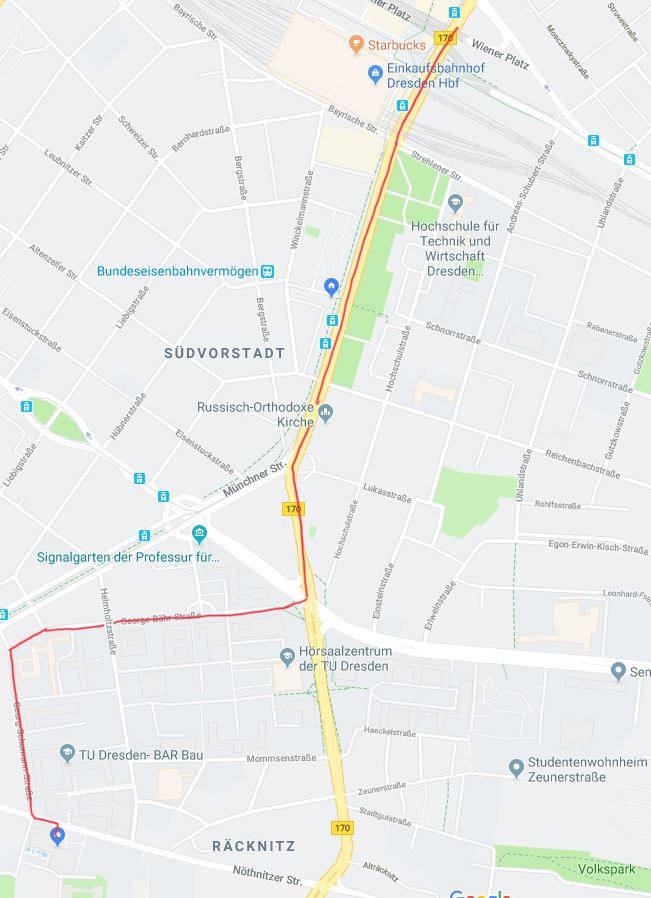
\includegraphics[width=\linewidth]{./toureins.jpg}
\newpage
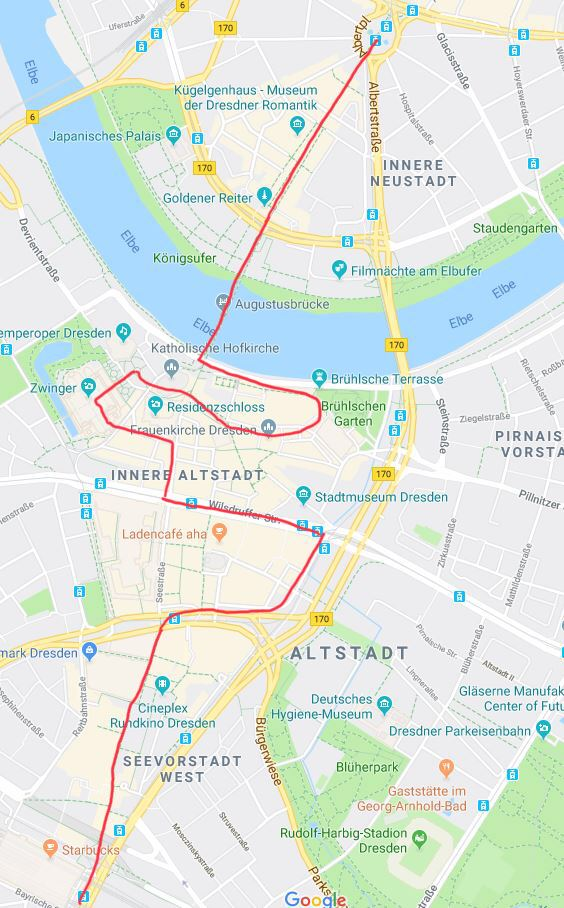
\includegraphics[width=\linewidth]{./tourzwei.jpg}
\chapter{Zu vermittelnde Informationen}

\section{1. Andreas-Pfitzmann-Bau}
\begin{itemize*}
\item Gründung der Fakultät Informatik 1969 - nächste Woche 50 Jahr Feier
\item Während der Tour werdet ihr merken, dass dieses Jahr viele Jubileumsfeiern anstehen
\item APB 2004 eröffnet
\item 2014 wurde es in Andreas-Pfitzmann-Bau umbenannt (ehmaliger Dekan der Fakultät)
\end{itemize*}

\section{2. Georg-Schuhmann-Bau}
\begin{itemize*}
\item War 1907 ehmaliges Landgericht, 1952 durch Bezirksgericht ersetzt
\item Heute sind noch 6 Todeszellen in dem Gebäude im ursprünglichen Zustand
\item Sie beherbergen heute eine kleine Ausstellung zur Geschichte des Landgerichts
\item Georg Schuhmann war Kommunist und Wiederstandskämpfer gegen den Nationalsozialismus
\item Er wurde am 11. Januar 1945 hingerichtet wegen Vorbereitung zum Hochverrat, Feindbegünstigung und Wehrkraftzersetzung“, da er nicht den Namen von anderen Wiederstandskämpfer preisgeben wollte
\item 
\item Die Gänge des Gebäudes sind sehr verwickelt und es ist wirklich schwer sich zurechtzufinden. Wenn man einen Raum sucht sollte man ca. 20min dafür einrechnen. Angeblich ist das wohl extra so gebaut worden, damit ausgebrochene Gefangene nicht aus dem Gebäude finden und flüchten können. Aus diesem Grund wird das Gebäude von den Studierenden auch liebevoll Hogwarts genannt, weil man das Gefühl bekommt, dass sich die Treppen bewegen und verschieben.
\end{itemize*}


\section{3. Stura/ Beyer-Bau}
\begin{itemize*}
	\item Vor dem Beyer-Bau stehn bleiben und kurz auf den Stura verweisen, der die Straße hoch liegt.
	\item Ein schlechten Witz reißen, weil die Stura-Barakae sehr unansehnlich ist und deswegen wird sie nicht gezeigt
	\item Der Stura feiert dieses Jahr sein 30 jähriges Bestehen
	\item Seit einem Monat trägt der Stura offiziell den Namen Studierendenrat und nicht mehr Studentenrat. Somit ist er einen der letzten Sturas der seinen Namen geändert hat.
	
	\item 
	\item Der Beyer-Bau wurde 1910 erbaut und beheimatet die Bauingeneurabteilung.
	\item Kurt Beyer war Bauigeneur und Hochschullehrer aus Dresden. 
	\item Außerdem beinhaltet es ein Observatorium, dass heute noch funktioniert
	\item Netter Sidefact: Es gibt eine Briefmarke mit dem Beyer-Bau
\end{itemize*}

Fritz-Löffler-Straße weiterlaufen. Richtung Hauptbahnhof.
Kann auf die Russisch orthodoxe Kirche und die Studentenwohnheime verweisen, so wie Club 11, Gag 18, Notivatis.

\section{4. Studentenwerk Dresden}
\begin{itemize*}
	\item Das Studentenwerk feiert dieses Jahr sein 100 jähriges bestehen
\end{itemize*}

\section{5. Russisch-orthodoxe Kirche}
\begin{itemize*}
	\item Errichtet zwischen 1872 und 1874 von dem Architekten Harald Julius von Bosse ist die Kirche des heiligen Simons auch heute noch Teil des Moskauer Patriarchs 
	\item Der Bau kostete 520.000 Reichsmark was aber leider nicht mehr für eine vernüftige Innenaustattung übrig ließ die dementsprechend weniger üppig ausfällt. 
	\item Die Kirche überstand die Luftangriffe 1945 als einziges Gebäude in der Umgebung heil. 
\end{itemize*}

\section{6. Hauptbahnhof}
\begin{itemize*}
	\item Größter Bahnhof Dresdens (duh) mit täglich ca. 60.000 Reisenden. 
   \item Nach Zerstörung 1945, Wiederaufbau. So entwickelte er sich in den 60ern zu einem bedeutenden Knotenpunkt für die Reise vom Westblock nach Südosteuropa. 
   \item Seit den 1990ern ist ein Modernisierungsvorhaben im Gange welches bis 2006 bereits 250 Millionen Euro kostete. Voraussichtliche Fertigstellung ist im nächsten Jahr wobei das noch fraglich ist. 
\end{itemize*}

\section{6. Pragerstraße}
\begin{itemize*}
	\item  Wurde 1945 stark zerstört. Wurde danach wiederaufgebaut und ist seit 1970 eine Fußgängerzone. Ist heute die bedeutendste Einkaufsstraße in Dresden.
\end{itemize*}

\section{7. Neues Rathhaus}
\begin{itemize*}
	\item Heutzutage Sitz der Dresdener Stadtverwaltung.
	\item wurde 1905-1910 erbaut nach einem Entwurf von Karl Roth. Funfacht: 1901 wurde ein Architekturwettbewerb für den Bau des Rathauses veranstaltet. Es wurden 4 Preise verliehen, aber kein 1. Platz.
	\item Das Rathaus wurde im Februar 1945 ebenfalls von Luftangriffen stark beschädigt.
	\item vor dem Gebäude steht die "Trümmerfrau"-Statue, sie soll an die Frauen erinnern, die die Stadt nach der Zerstörung reinigten und den Schutt beseitigten.
\end{itemize*}

\section{8. Altmarkt}
\begin{itemize*}
\item ältester Platz Dresdens, hat den Namen seit fast 500 Jahren nach Entstehung des Neumarkts
\item schon immer umgeben von Wohn- und Geschäftshäusern und wichtigen Straßen
\item hier wurden nach dem Bombenagriff am 13. Februar 1945 fast 7.000 Leichen verbrannt
\item Platz für diverse Veranstaltungen über das Jahr hinweg (z.B. Striezelmarkt, einer der ältesten deutschen Weihnachtsmärkte)
\item Im Süden (schräg): Kreuzkirche
    \begin{itemize*}
    \item Größte Kirche Sachsen (über 3.000 Plätze)
    \item Mehrmals zerstört und immer wieder aufgebaut (zuletzt im 2. Weltkrieg)
    \end{itemize*}
\item Im Norden: Kulturpalast
    \begin{itemize*}
    \item Mehrzwecksaal der 1969 eingeweiht wurde; z.B. Konzerte der Philharmonie
    \item Wurde vor Kurzem umgebaut um eine bessere Akkustik zu gewährleisten (Wiedereröffnung April 2017)
    item An der Seite des Kulturpalast: Wandbild „Weg der roten Fahne“, mittlerweile Kulturdenkmal
    \end{itemize*}
\end{itemize*}

\section{9. Residenzschloss}
\begin{itemize*}
\item war das Residenzschloss der sächsischen Kurfürsten (1547–1806) und Könige (1806–1918)
\item eines der ältesten Bauwerke der Stadt und baugeschichtlich bedeutsam, da alle Stilrichtungen von Romanik bis Historismus vertreten sind
\item brannte im 2. WK bis auf Grundmauern nieder, Wiederaufbau ab 1985
    \begin{itemize*}
    \item 1991 bekam der Hausmannsturm seine Spitze zurück
    \item 2004 Einrichtung der Kunstbibliothek, des Kupferstichkabinetts und des Neuen Grünen Gewölbes
    \item 2006 Historisches Grünes Gewölbe
    \item 2010 Türckische Kammer
    \end{itemize*}
\item beherbergt heute fünf Museen:
    \begin{itemize*}
    \item Historisches und Neues Grünes Gewölbe
    \item Münzkabinett
    \item Kupferstichkabinett
    \item Rüstkammer Türckische Kammer
    \end{itemize*}
\end{itemize*}
\subsection{Sidefacts Residenzschloss}
\begin{itemize*}
\item nach dem 2. WK wurde in einem Teil der Kellergewölbe einige Jahre lang eine Pilzzucht betrieben
\item in den ersten Jahren nach Wiedereröffnung des Hist. Gr. Gewölbe musste man Tickets lange im Voraus kaufen (bis zu einem Jahr)
\item bei Caterings im Innenhof ist der Ausschank von Rotwein (meistens) verboten, wegen des Sandsteinbodens
\end{itemize*}

Nur wenn Zeit ist:
\section{10. Cholerabrunnen}
\begin{itemize*}
\item auch Gutschmid-Brunnen, von Freiherr Eugen von Gutschmid finanziert
\item sollte Dank ausdrücken, dass Dresden Mitte des 19. Jahrh. von der Cholera verschont wurde
\end{itemize*}

\section{11. Zwinger}
\begin{itemize*}
\item 1709-1732 von bedeutendem Architekten Pöppelmann erbaut
\item im Auftrag von August dem Starken, der die Künste und das Vergnügen jeglicher Art liebte und gern wie Ludwig XIV sein wollte, aber weder ein großer Kriegsherr noch ein großer Politiker war, und auch nicht besonders gut mit Geld umgehen konnte
\item als Festplatz für die Hofgesellschaft gedacht, außerdem als Orangerie für die Orangenbäume
\item der Name „Zwinger“ kommt daher, da der Raum zwischen der äußeren und der inneren Festungsmauer als Zwinger bezeichnet wurde
\item August III war noch vernarrter in die Kunst als sein Vater, sodass er mit dem Architekten Gottfried Semper die vierte Seite des Zwingers als Gemäldegalerie bauen ließ (die „Alten Meister“)
\item Zwinger beherbergt neben Gemäldegalerie noch die kurfürstliche Porzellansammlung und den mathematisch-physikalischen Salon
\item das „Nymphenbad“, ein barocker Brunnen (verlassen des Zwingers durch das Nymphenbad)
\item jede Viertelstunde kann man das Porzellanglockenspiel hören
\end{itemize*}

\section{12. Semperoper / Theaterplatz}
\begin{itemize*}
\item ist das Opernhaus der Sächsischen Staatsoper Dresden
\item die Dresdner Phillharmoniker gelten als eines der besten Orchester der Welt
\item nach ihrem Architekten Gottfried Semper benannt
\item 1871-1878 erbaut (nachdem 1869 das vorherige Theaterhaus abgebrannt ist)
\item nach Entwurf von G. Semper, aber unter Leitung seines Sohnes gebaut (er war im Exil)
\item im 2. WK komplett zerstört - ab 1977 Wiederaufbau
\item am 13. Februar 1985 (40. Jahrestag der kriegsbedingten Zerstörung) konnte die Semperoper mit Carl Maria von Webers Oper Der Freischütz wiedereröffnet werden (mit dieses Werk wurde das Opernhaus am 31. August 1944 geschlossen)
\item auf/an Theaterplatz:
    \begin{itemize*}
    \item bronzene Reiterstandbild des sächsischen Königs Johann (1889 geschaffen)
    \item Brunnen und Carl-Maria-von-Weber-Denkmal
    \item Italienisches Dörfchen
    \end{itemize*}
\end{itemize*}
\subsection{Sidefacts Semperoper / Theaterplatz}
\begin{itemize*}
\item weil die Semperoper in der Radeberger Bier Werbung zu sehen ist, denken viele es wäre die Brauerei
\item in der Zeit des Nationalsozialismus hieß der Theaterplatz Adolf-Hitler-Platz
\end{itemize*}

Nur wen Zeit
\section{13. Kathedrale (Hofkirche)}
\begin{itemize*}
\item ist Kathedrale des Bistums Dresden-Meißen (seit 1980) sowie eine Stadtpfarrkirche Dresdens
\item unter Kurfürst Friedrich August II. von Sachsen (durch Gaetano Chiaveri) von 1739 bis 1755 im Stil des Barocks errichtet
\item ist durch einen Übergang mit dem Residenzschloss verbunden
\item wurde im 2. WK stark zerstört, aber schon ab Juni 1945 wieder für Messen genutzt (Bennokapelle, dann linker Seitenflügel) ab 1962 konnte sie wieder komplett genutzt werden
\end{itemize*}
\subsection{Sidefacts Kathedrale}
\begin{itemize*}
\item Hauptgrund für Bau: Sachsen war zwar evangelisch, aber eine katholische Kirche wurde in Dresden benötigt, weil August der Starke König von Polen werden wollte (musste als König ebenfalls katholisch werden)
\item in Grabgewölben wurden viele Wettiner Könige + Familie beigesetzt, das Herz August des Starken befindet sich hier in einer Kapsel in der Stiftergruft
\end{itemize*}

\section{14. Fürstenzug}
\begin{itemize*}
\item besteht aus ca. 23000 Fliesen aus Meißner Porzellan
\item 102 Meter lang
\item zeigt Ahnengalerie von 1127 bis 1904 - Grafen, Herzoge, Kurfürsten und Könige
\item während des 2. WK nur mininmal zerstört, da das Porzellan den hohen Temperaturen standhalten konnte
\end{itemize*}

\section{15. Frauenkirche}
\begin{itemize*}
\item das bekannteste Wahrzeichen der Stadt
\item wurde im 2. Weltkrieg zerstört, aber nicht durch Bomben
    \begin{itemize*}
    \item diese prallten von der Kuppel ab, aber die hohen Temperaturen durch den Feuersturm machten den Sandstein spröde, so dass sie 2 Tage später zusammenbrach
    \item Zerstörung war für Dresdner von hoher Symbolkraft, da damit auch der letzte Teil des alten Dresdens zerstört war
    \end{itemize*}
\item in der DDR diente die Ruine als Mahnmal gegen den Krieg
\item 2005 wurde der ausschließlich durch Spenden finanzierte Wiederaufbau beendet
\item einzigartig auf der Welt: die am unteren Ende nach innen gewölbte Kuppel - ähnlich einer Glocke
\item schwarze Steine sind Steine der alten Kirche (insgesamt 43\% der Kirche), allerdings keine in Kuppel wiederverwendet, da hohe Stabilität enorm wichtig ist
\item das Kreuz wurde von Sohn eines britischen Bomberpilots gefertigt, der auch die Angriffe auf Dresden flog
\end{itemize*}

\section{16. Festung Dresden}
\begin{itemize*}
\item 1299 erstmals erwähnt
\item umfasste Innere Altstadt (Prager Straße) bis Innere Neustadt (Albertplatz bzw. 300m nördlich vom goldenen Reiter)
\item es gab fünf Stadttore, meherere Bastionstürme und Mauertürme
\item entfestigt und zurückgebaut bis 1811, heute sind kaum noch Befestigungsanlagen zu erkennen
\item seit 1992 Museum im erhaltenen Teil der Dresdner Befestigungsanlagen
\end{itemize*}

\section{17. Brühlsche Terassen und Umgebung}
\begin{itemize*}
\item der „Balkon Europas“ genannt - wegen des schönen Ausblicks auf die Elbe und der Tatsache, dass sich viele historisch wichtige Gebäude an ihr entlang aufreihen, zb das Albertinum, das Johanneum und die Kunstakademie (auch als „Zitronenpresse“ bezeichnet)
\item Graf Brühl machte den Festungswall im 18. Jh zu seinem privaten Lustgarten
\item Elbwiesen mit Filmnächten (Konzerte und Filme im Sommer)
\item Sächsische Dampfschifffahrt
    \begin{itemize*}
    \item älteste/größte Raddampferflotte der Welt
    \item 9 Raddampfer, 7 davon aus den Jahren 1879-1898
    \item Linienfahrten bis Bad Schandau, Tourismusfahrten
    \end{itemize*}
\item zwei „Jahrhunderthochwasser“ (2002 und 2013) der Elbe mit vielen Schäden in ganz Dresden und Umgebung
\end{itemize*}

\section{18. Augustusbrücke}
\begin{itemize*}
\item erste und älteste Steinbrücke über die Elbe, löst 1275 eine Holzkonstruktion ab und gehört dann mit den damals 25 Bögen zu den längsten Brücken in ganz Deutschland
\item 1729 war es August der Starke, der eine Erweiterung der Brücke vornehmen ließ (wiederum von Pöppelmann), da der zunehmende Verkehr zu viel für die Brücke wurde - erbaute eine der prächtigsten und schönsten Brücken in ganz Europa nach dem Vorbild der Karlsbrücke in Prag
\item kompletter Neubau 1907, da sie für die Straßenbahnen zu eng und für die Schiffe zu niedrig wurde, jedoch nahm man wieder Sandstein und orientierte sich an Pöppelmanns Entwürfen
\item gegen Ende es zweiten Weltkriegs - völlig sinnlos - zu Teilen gesprengt und danach wieder errichtet
\item noch fahren Autos darüber, was in ein paar Jahren aber nicht mehr so sein wird: wenn 2016 die Albertbrücke wieder befahrbar ist, soll die Augustusbrücke für immer kraftfahrzeugfreie Zone werden
\end{itemize*}

\section{19. Japanisches Palais}
\begin{itemize*}
\item Museum für Völkerkunde und Naturhistorische Sammlungen
\item Highlight: Damaskuszimmer - prunkvoll verzierter Empfangsraum eines Damaszener Wohnhauses
\item früher Kurfürstliche Bibliothek, woraus später hauptsächlich die Sächsische Landesbibliothek hervorging
\item 1715 von Rudolph Faesch für Jakob Heinrich Graf von Flemming errichtet (kleineres Landhaus -nicht mehr erkennbar)
\item August der Starke hegte großes Interesse an dem Palais
\item 1727 bis 1733 Umbau in heutige Form (fast komplett) - Name dort erhalten
\item Zerstörungen im im 7jährigen Krieg und 2. WK
\end{itemize*}

\section{20. Goldener Reiter}
\begin{itemize*}
\item 1736 wurde das Denkmal enthüllt (3 Jahre nach dem Tod von August dem Starken)
\item ehemals feuervergoldet, später mit Blattgold restauriert
\item (evtl. Informationen zur Neustadt geben als Abschluss)
\end{itemize*}

Weiterlaufen Richtung Albertplatz.

\end{document}
